\chapter{Wie komplexe Zahlen Struktur erzeugen}
\label{chap:VII_komplexe Struktur}


\subsection{Iteration als mathematisches Prinzip}

\index{Iteration}
\index{Dynamisches System}
\index{Abbildung}

Iteration ist eines der einfachsten und zugleich mächtigsten Prinzipien der Mathematik:
Man nimmt eine Vorschrift, wendet sie an – und wendet das Ergebnis wieder auf dieselbe Vorschrift an.
Aus einer einzigen Regel entsteht eine Folge von Zuständen. Genau hier beginnt „Struktur aus Mathematik“.

Formal betrachtet ist Iteration die wiederholte Anwendung einer Abbildung $f$:
\[
z_{0},\quad z_{1}=f(z_{0}),\quad z_{2}=f(z_{1})=f(f(z_{0})),\quad \ldots,\quad z_{n+1}=f(z_n).
\]
Damit wird aus einer Zahl $z_0$ eine ganze Bahn durch den Zustandsraum.
\index{Orbit}

\subsubsection*{Ein wirkliches Zahlenbeispiel (damit das Schema greifbar wird)}
Nehmen wir eine extrem einfache Funktion auf den reellen Zahlen:
\[
f(x)=\frac12 x + 1.
\]
Wir starten mit $x_0=0$ und wenden immer wieder dieselbe Vorschrift an:
\[
\begin{aligned}
	x_1 &= f(x_0)=1,\\
	x_2 &= f(x_1)=1{,}5,\\
	x_3 &= f(x_2)=1{,}75,\\
	x_4 &= 1{,}875,\\
	x_5 &= 1{,}9375,\\
	x_6 &= 1{,}96875.
\end{aligned}
\]
Man sieht sofort: Die Folge nähert sich einer festen Zahl an, nämlich $2$.
Diese Zahl ist ein \emph{Fixpunkt}, denn $f(2)=2$ gilt.
\index{Fixpunkt}

\begin{DidacticBox}[Was man hier wirklich lernen soll]
	\index{Iteration}
	Iteration bedeutet nicht „eine Rechnung“, sondern \emph{eine Regel in der Zeit}:
	Aus $x_0$ wird $x_1$, daraus $x_2$, daraus $x_3$.
	Schon bei einer simplen Vorschrift entstehen typische Verhaltensweisen:
	\emph{Annäherung} (stabil), \emph{Schwanken} (periodisch) oder \emph{Weglaufen} (divergent).
\end{DidacticBox}

Diese Sicht ist entscheidend: Zahlen werden zu Zuständen, und die Funktion $f$ wird zur Dynamik.
Damit ist Iteration bereits ein dynamisches System – im reinsten, abstraktesten Sinn.
\index{Dynamisches System}

\begin{MathBox}[Begriffe: Orbit und Fixpunkt]
	\index{Orbit}
	\index{Fixpunkt}
	Gegeben sei $f:\mathbb{C}\to\mathbb{C}$ und ein Startwert $z_0\in\mathbb{C}$.
	Die Iteration ist
	\[
	z_{n+1}=f(z_n)\qquad (n=0,1,2,\dots).
	\]
	Die Folge $(z_0,z_1,z_2,\dots)$ heißt \emph{Orbit} (Bahn) von $z_0$.
	Ein Punkt $z^\ast$ heißt \emph{Fixpunkt}, wenn $f(z^\ast)=z^\ast$ gilt.
\end{MathBox}

\subsubsection*{Warum komplexe Zahlen hier etwas Besonderes sind}
\index{Komplexe Zahl}
\index{Komplexe Ebene}
In $\mathbb{R}$ läuft eine Iteration entlang einer Zahlengeraden. In $\mathbb{C}$ bewegt sie sich in einer Ebene.
Allein dieser Schritt verändert alles: Bahnen können kreisen, spiralförmig streben, Grenzen ausbilden,
Inseln erzeugen und feine Ränder entwickeln. Aus einer Vorschrift wird Geometrie.

Für die späteren Bilder (Mandelbrot- und Julia-Mengen) genügt im Kern eine einzige Familie:
\[
f_c(z)=z^2+c \qquad (z,c\in\mathbb{C}).
\]
Wir starten bei einem $z_0$ und verfolgen die Iteration. Die Leitfrage ist dabei brutal simpel:
\emph{Bleibt die Bahn beschränkt oder fliegt sie ins Unendliche?}

\subsubsection*{Kurzfazit}
\begin{itemize}
	\item Iteration heißt: dieselbe Vorschrift immer wieder anwenden.
	\item Das erzeugt Bahnen (Orbits) mit qualitativ verschiedenem Verhalten: stabil, periodisch oder divergent.
	\item In der komplexen Ebene wird dieses Verhalten sichtbar als Form.
\end{itemize}

\noindent\textbf{Übergang:} Im nächsten Abschnitt klären wir präzise, was „beschränkt“ und „divergent“ bedeutet
und warum genau der Grenzbereich zwischen beidem später die Struktur trägt.

\subsection{Stabilität, Divergenz und Grenzfälle}
\index{Stabilität}
\index{Divergenz}
\index{Grenzfall}
\index{Orbit}

Wenn wir eine Iteration $z_{n+1}=f(z_n)$ betrachten, dann ist die zentrale Frage nicht „Welche Zahl kommt als nächste?“,
sondern: \emph{Was passiert langfristig?}
Bleibt die Bahn in einem begrenzten Bereich, oder läuft sie davon?
Diese einfache Unterscheidung trennt stabile von instabilen Dynamiken.

\subsubsection*{Stabilität: Bahnen bleiben in der Nähe}
Im stabilen Fall ist ein Startwert „robust“: Kleine Änderungen am Startwert verändern zwar die Folge,
aber nicht ihr qualitatives Verhalten. Man kann sich das so vorstellen:
Die Iteration zieht Bahnen in einen bestimmten Bereich hinein, statt sie hinauszutreiben.
Typisch ist dabei die Annäherung an einen Fixpunkt oder an einen periodischen Zyklus.
\index{Fixpunkt}
\index{Periode}

\subsubsection*{Divergenz: Bahnen fliegen weg}
Im instabilen Fall passiert das Gegenteil: Die Iteration verstärkt Abweichungen.
Die Folge wächst im Betrag immer weiter, sie „entkommt“ aus jedem beschränkten Bereich.
Genau dieses Verhalten werden wir später als Kriterium verwenden: \emph{Wer wegfliegt, gehört nicht zur Struktur.}
\index{Betrag}
\subsubsection*{Zwei Mini-Beispiele: stabil vs.\ divergent}
\index{Stabilität}
\index{Divergenz}

\begin{figure}[h]
	\centering
	
	\begin{tikzpicture}
		\begin{axis}[
			width=0.46\textwidth,
			height=4.2cm,
			xlabel={$n$},
			ylabel={$x_n$},
			title={Stabil: $x_{n+1}=\tfrac12 x_n+1$},
			ymin=0, ymax=2.1,
			xtick={0,1,2,3,4,5,6,7,8},
			ytick={0,0.5,1,1.5,2}
			]
			\addplot+[mark=*] coordinates {
				(0,0)
				(1,1)
				(2,1.5)
				(3,1.75)
				(4,1.875)
				(5,1.9375)
				(6,1.96875)
				(7,1.984375)
				(8,1.9921875)
			};
		\end{axis}
	\end{tikzpicture}
	\hfill
	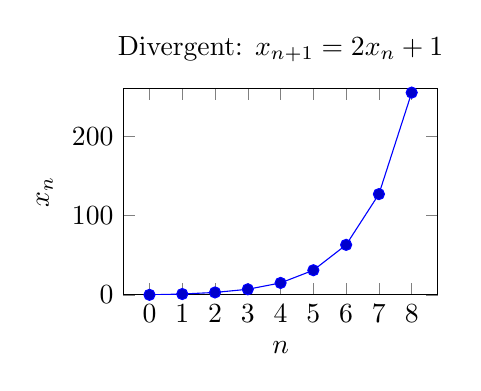
\begin{tikzpicture}
		\begin{axis}[
			width=0.46\textwidth,
			height=4.2cm,
			xlabel={$n$},
			ylabel={$x_n$},
			title={Divergent: $x_{n+1}=2x_n+1$},
			ymin=0, ymax=260,
			xtick={0,1,2,3,4,5,6,7,8}
			]
			\addplot+[mark=*] coordinates {
				(0,0)
				(1,1)
				(2,3)
				(3,7)
				(4,15)
				(5,31)
				(6,63)
				(7,127)
				(8,255)
			};
		\end{axis}
	\end{tikzpicture}
	
\end{figure}
\begin{DidacticBox}[Stabil vs.\ chaotisch: nicht verwechseln]
	\index{Chaos}
	Stabilität bedeutet nicht „langweilig“, und Instabilität bedeutet nicht automatisch „Zufall“.
	Auch chaotische Bahnen sind deterministisch, aber sie sind empfindlich gegenüber kleinsten Änderungen.
	Für unsere Zwecke reicht zunächst eine robustere Leitidee:
	\emph{beschränkt} versus \emph{unbeschränkt}.
	Der Grenzbereich zwischen beidem ist später der Ort der sichtbaren Struktur.
\end{DidacticBox}

\subsubsection*{Beschränktheit als Kriterium}
In der komplexen Ebene ist es besonders natürlich, den \emph{Betrag} $|z_n|$ zu betrachten.
Wir nennen einen Orbit \emph{beschränkt}, wenn es eine Zahl $R>0$ gibt, so dass
\[
|z_n|\le R \quad \text{für alle } n.
\]
Existiert kein solches $R$, dann läuft der Orbit ins Unendliche: $|z_n|\to\infty$.

\begin{MathBox}[Beschränkt oder unbeschränkt]
	\index{Beschränktheit}
	\index{Betrag}
	Für die Iteration $z_{n+1}=f(z_n)$ heißt der Orbit von $z_0$ \emph{beschränkt}, wenn
	\[
	\exists\, R>0:\ \forall n\in\mathbb{N}\ \ |z_n|\le R.
	\]
	Ist das nicht der Fall, nennt man den Orbit \emph{unbeschränkt} (oder divergent);
	typisch ist dann $|z_n|\to\infty$.
\end{MathBox}
\subsubsection*{Ein einfaches komplexes Beispiel: Spiralbahn im Kreis}
Wir betrachten die Iteration
\[
z_{n+1}=a\,z_n,\qquad a=0{,}85\,e^{i\pi/5},\qquad z_0=2+i.
\]
Da $|a|=0{,}85<1$ gilt
\[
|z_n|=|a|^n|z_0|\le |z_0|=:R=\sqrt{5}.
\]
Der Orbit bleibt also für alle $n$ im Kreisradius $R$ und spiralt gegen $0$.

\begin{figure}[h]
	\centering
	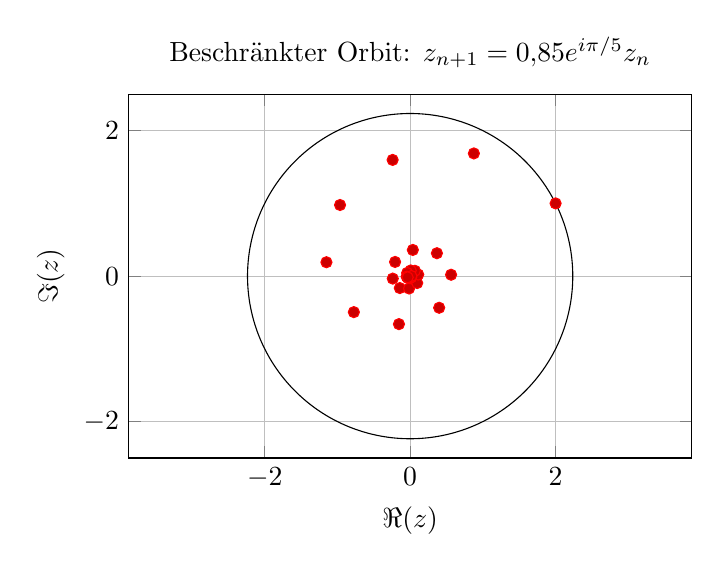
\begin{tikzpicture}
		\begin{axis}[
			axis equal,
			width=0.72\textwidth,
			height=6.2cm,
			xlabel={$\Re(z)$},
			ylabel={$\Im(z)$},
			title={Beschränkter Orbit: $z_{n+1}=0{,}85e^{i\pi/5}z_n$},
			xmin=-2.5, xmax=2.5,
			ymin=-2.5, ymax=2.5,
			grid=both
			]
			% Kreisradius R = sqrt(5)
			\addplot[domain=0:360, samples=361] ({sqrt(5)*cos(x)},{sqrt(5)*sin(x)});
			
			% Orbitpunkte (n=0..25)
			\addplot+[only marks, mark=*] coordinates {
				(2.000,1.000)
				(0.876,1.687)
				(-0.241,1.598)
				(-0.964,0.978)
				(-1.151,0.191)
				(-0.774,-0.495)
				(-0.154,-0.660)
				(0.399,-0.435)
				(0.563,0.019)
				(0.368,0.315)
				(0.037,0.360)
				(-0.207,0.195)
				(-0.239,-0.034)
				(-0.142,-0.164)
				(-0.015,-0.170)
				(0.097,-0.095)
				(0.111,0.022)
				(0.066,0.073)
				(0.008,0.078)
				(-0.041,0.044)
				(-0.048,-0.007)
				(-0.030,-0.026)
				(-0.005,-0.028)
				(0.015,-0.016)
				(0.017,0.002)
				(-0.034,-0.017)
			};
		\end{axis}
	\end{tikzpicture}
\end{figure}
\subsubsection*{Der Grenzfall: die eigentliche Bühne der Struktur}
Jetzt kommt der entscheidende Punkt für das ganze Kapitel:
Zwischen eindeutig stabil und eindeutig divergent liegt ein Randbereich, der extrem empfindlich ist.
Startwerte, die nur minimal voneinander abweichen, können völlig verschieden enden:
Der eine Orbit bleibt beschränkt, der andere fliegt weg.
Dieser „Übergang“ ist kein Nebeneffekt, sondern das Zentrum des Phänomens.

Genau deshalb entstehen später scharfe, fransige Grenzen und scheinbar unendliche Detailtiefe.
Nicht weil wir Natur modellieren, sondern weil wir eine mathematische Grenzfrage stellen.
\subsubsection*{Grenzfall: eine minimale Änderung entscheidet alles}
Wir betrachten die Iteration
\[
z_{n+1}=z_n^2,
\]
also die Quadratik $f(z)=z^2$. Hier lässt sich der Grenzfall vollständig verstehen:
\emph{Die Grenze zwischen beschränkt und unbeschränkt ist der Einheitskreis $|z|=1$.}
Damit ist bereits sichtbar, was später bei Mandelbrot- und Julia-Mengen in viel komplizierterer Form auftritt:
Ein Randbereich entscheidet über „bleibt drin“ oder „fliegt weg“.

Wir wählen zwei fast identische Startwerte:
\[
z_0=0{,}99 \quad (\text{knapp innerhalb}), 
\qquad z_0=1{,}01 \quad (\text{knapp außerhalb}).
\]

\begin{figure}[h]
	\centering
	
	% --- Bild links: komplexe Ebene mit Einheitskreis und Startpunkten ---
	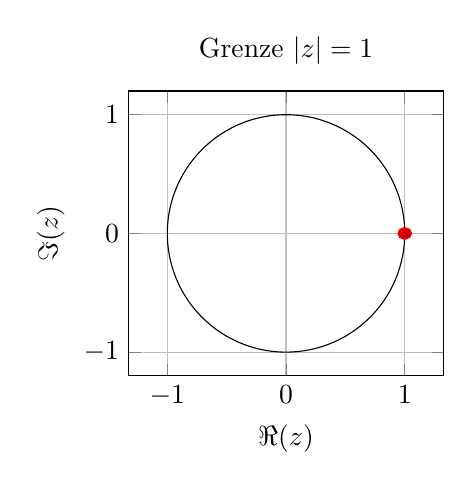
\begin{tikzpicture}
		\begin{axis}[
			axis equal,
			width=0.46\textwidth,
			height=5.2cm,
			xlabel={$\Re(z)$},
			ylabel={$\Im(z)$},
			title={Grenze $|z|=1$},
			xmin=-1.2, xmax=1.2,
			ymin=-1.2, ymax=1.2,
			grid=both
			]
			% Einheitskreis
			\addplot[domain=0:360, samples=361] ({cos(x)},{sin(x)});
			% Startpunkte
			\addplot+[only marks, mark=*] coordinates {(0.99,0) (1.01,0)};
		\end{axis}
	\end{tikzpicture}
	\hfill
	% --- Bild rechts: Betrag als Funktion von n (log-Skala) ---
	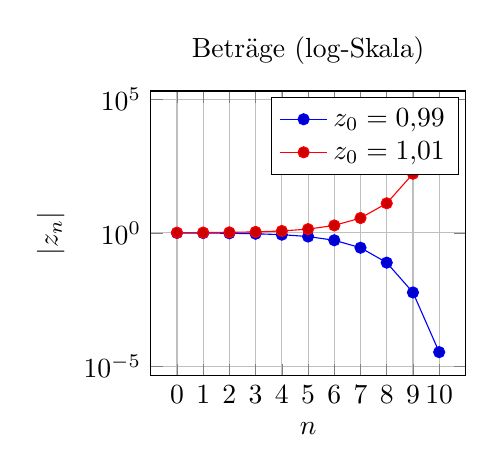
\begin{tikzpicture}
		\begin{axis}[
			width=0.46\textwidth,
			height=5.2cm,
			xlabel={$n$},
			ylabel={$|z_n|$},
			title={Beträge (log-Skala)},
			ymode=log,
			log basis y={10},
			xtick={0,1,2,3,4,5,6,7,8,9,10},
			grid=both
			]
			% z0=0.99
			\addplot+[mark=*] coordinates {
				(0,0.99)
				(1,0.9801)
				(2,0.96059601)
				(3,0.9227446944)
				(4,0.8514577711)
				(5,0.7249803360)
				(6,0.5255964875)
				(7,0.2762516677)
				(8,0.0763149839)
				(9,0.0058239768)
				(10,0.0000339187)
			};
			\addlegendentry{$z_0=0{,}99$}
			
			% z0=1.01
			\addplot+[mark=*] coordinates {
				(0,1.01)
				(1,1.0201)
				(2,1.04060401)
				(3,1.0828567056)
				(4,1.1725786449)
				(5,1.3749406785)
				(6,1.8904618695)
				(7,3.5738460800)
				(8,12.7723758032)
				(9,163.1335836586)
				(10,26612.5661173053)
			};
			\addlegendentry{$z_0=1{,}01$}
		\end{axis}
	\end{tikzpicture}
	
	\caption{Grenzfall bei $z_{n+1}=z_n^2$: Innerhalb des Einheitskreises bleiben Bahnen beschränkt, außerhalb divergieren sie. Schon eine minimale Änderung des Startwerts kann das Verhalten vollständig kippen.}
\end{figure}
\subsubsection*{Vorbereitung auf die Quadratik $z^2+c$}
\index{Quadratische Abbildung}
Für die Familie $f_c(z)=z^2+c$ wird es sogar ein praktisches Kriterium geben:
Wenn der Betrag eines Orbit irgendwann groß genug wird, dann ist sicher, dass er weiter wächst und entkommt.
Damit lässt sich „dazugehörig“ versus „nicht dazuzugehörig“ rechnerisch entscheiden.

\noindent\textbf{Übergang:} Im nächsten Abschnitt verwenden wir genau diese Idee als Landkarte:
Für welche Parameter $c$ bleibt der Orbit von $z_0=0$ beschränkt?
Die Antwort ist die Mandelbrot-Menge.

%------------------------------------------------------------
\subsection{Die Mandelbrotmenge als Landkarte}
\label{sec:VII-7-3}

\index{Mandelbrotmenge}
\index{Parameterraum}
\index{komplexe Ebene}
\index{Iteration}
\index{Beschränktheit}
\index{Divergenz}
\index{Stabilität}
\index{Fraktal}
\index{Selbstähnlichkeit}
\index{Fluchtzeit}
\index{Escape-Radius}

\textbf{Leitfrage:} \emph{Wie liest man die Mandelbrotmenge wie eine Landkarte – und was bedeuten „Land“, „Meer“ und „Küste“ mathematisch?}

Die Mandelbrotmenge ist keine Bahnkurve einer einzelnen Rechnung. Sie ist eine \emph{Landkarte im Parameterraum}:
Jeder Punkt \(c\) in der komplexen Ebene steht für ein eigenes Iterationssystem. Das Bild ordnet also nicht Werte \(z_n\),
sondern \emph{Systeme nach ihrem Verhalten}.

\begin{MathBox}[Definition: Landkarte im Parameterraum]
	Wir betrachten die Iteration
	\[
	z_{n+1} = z_n^2 + c, \qquad z_0 = 0, \qquad c\in\mathbb{C}.
	\]
	Die \textbf{Mandelbrotmenge} ist die Menge aller Parameter \(c\), für die die Folge \(\{z_n\}\) \textbf{beschränkt} bleibt:
	\[
	\mathcal{M}=\{\,c\in\mathbb{C}\mid \sup_n |z_n| < \infty\,\}.
	\]
\end{MathBox}

\begin{DidacticBox}[Der häufigste Denkfehler]
	In der Grafik ist \textbf{nicht} \(z\) die Koordinate, sondern der Parameter \(c\).
	Für \emph{jeden} Bildpunkt wird dieselbe Iteration gestartet (immer \(z_0=0\)), aber mit anderem \(c\).
	Darum ist das Bild eine \textbf{Landkarte}: Jeder Punkt entspricht einem eigenen Dynamik-„Universum“.
\end{DidacticBox}

\subsubsection*{Land, Meer und Küste}
Die Landkarten-Metapher ist nicht nur hübsch, sie ist präzise:

\begin{itemize}
	\item \textbf{Land (innen, oft schwarz):} \(\{z_n\}\) bleibt beschränkt \(\Rightarrow c\in\mathcal{M}\).
	\item \textbf{Meer (außen, farbig):} \(\{z_n\}\) entweicht \(\Rightarrow\) Divergenz.
	\item \textbf{Küste (Grenze):} Übergangsgebiet, in dem kleinste Änderungen in \(c\) das Verhalten kippen lassen.
\end{itemize}

\begin{NoteBox}[Fluchtkriterium und Einfärbung]
	Für \(z_{n+1}=z_n^2+c\) gilt: Sobald \(|z_n|>2\), ist Divergenz sicher (\textbf{Escape-Radius} \(2\)).
	Außerhalb der Menge zeigt die Farbgebung meist die \textbf{Fluchtzeit}:
	wie viele Iterationen bis \(|z_n|>2\) erreicht ist. Das ist Visualisierung, nicht Definition.
\end{NoteBox}

\subsubsection*{Die Grenze als „Bühne der Struktur“}
Der eigentliche Kern der Mandelbrotmenge ist nicht das „Innen“ oder „Außen“, sondern die \textbf{Grenze}:
Dort sitzt die gesamte Komplexität. Winzige Parameteränderungen entscheiden über Beschränktheit oder Divergenz.
Beim Hineinzoomen erscheinen immer neue Strukturen – das ist das typische Merkmal fraktaler Geometrie.

\begin{figure}[htbp]
	\centering
	% Datei anpassen:
	\includegraphics[width=0.88\linewidth]{Bilder/Mandelbrot.png}
	\caption{Die Mandelbrotmenge als Landkarte im Parameterraum \(c\): innen beschränkt (Land),
		außen Fluchtzeit-Färbung (Meer), die Grenze als strukturreiches „Küstengebiet“.}
	\label{fig:mandelbrot_landkarte}
\end{figure}

\subsubsection*{Merksätze}
\begin{itemize}
	\item Das Bild ist ein \textbf{Parameterraum}: Jeder Punkt ist ein eigenes Iterationssystem.
	\item \textbf{Innen} bedeutet: beschränkt \(\Rightarrow c\in\mathcal{M}\).
	\item \textbf{Farben außen} zeigen meist die \textbf{Fluchtzeit} (Hilfsmittel).
	\item Die \textbf{Grenze} ist das entscheidende Gebiet: dort entsteht die Detailtiefe.
\end{itemize}
Eine detaillierte, nachvollziehbare Erzeugung der Mandelbrot-Grafik (Pixel \(\to c\), Iteration, Fluchtzeit und Farbgebung)
findet sich in Anhang~\ref{app:mandelbrot-rendering}.

\medskip
\noindent\textbf{Übergang zu 7.4:} Jetzt wird die „Landkarte“ praktisch: Wir schauen auf Stabilität, Divergenz und Grenzfälle.
Dazu wählen wir konkrete Parameter \(c\) (klar \emph{innen}, klar \emph{außen}, und knapp an der Grenze) und sehen,
wie die Iteration sichtbar kippt.
%------------------------------------------------------------
\subsection{Julia-Mengen: lokale Dynamik und Struktur}
\label{sec:julia-mengen}
\index{Julia-Menge}
\index{komplexe Dynamik}
\index{Iteration}
\index{Mandelbrot-Menge}

\textbf{Leitfrage:} Was passiert \emph{lokal} im $z$-Raum, wenn der Parameter $c$ fest ist – und warum entstehen dabei so unterschiedliche, oft fraktale Grenzen?

Die Mandelbrotmenge aus Abschnitt~\ref{sec:VII-7-3} ist eine \emph{Landkarte des Parameterraums} (jedes $c$ ein Punkt).
Julia-Mengen sind die passende \emph{Landkarte des Zustandsraums}: Für ein \emph{festes} $c$ betrachten wir die Bahn eines Startwerts $z_0$ unter Iteration.
So wird aus „wo liegt $c$?“ die Frage „welche Startwerte $z_0$ bleiben gebunden – und welche fliegen davon?“.

\begin{MathBox}[Definition: Iteration, gefüllte Julia-Menge, Julia-Rand]
	\index{gef\"ullte Julia-Menge}
	\index{Fixpunkt}
	\index{Attraktor}
	Wir betrachten die quadratische Iteration
	\[
	z_{n+1}=f_c(z_n)=z_n^2+c \qquad (c\in\mathbb{C} \ \text{fest}).
	\]
	\begin{itemize}
		\item Die \emph{Bahn} von $z_0$ ist die Folge $(z_n)_{n\ge 0}$.
		\item Die \emph{gef\"ullte Julia-Menge} ist
		\[
		K_c=\{z_0\in\mathbb{C}\mid (z_n)\ \text{bleibt beschr\"ankt}\}.
		\]
		\item Die \emph{Julia-Menge} ist der Rand
		\[
		J_c=\partial K_c.
		\]
	\end{itemize}
	Anschaulich: $K_c$ sind die „Startwerte, die nicht explodieren“; $J_c$ ist die scharfe, fraktale Grenze zwischen gebunden und divergent.
\end{MathBox}

\subsubsection*{Lokale Dynamik: Stabilit\"at, Flucht und empfindliche Grenzen}
\index{Stabilit\"at}
\index{Divergenz}
Für viele Startwerte entscheidet sich das Schicksal schnell: Entweder die Folge bleibt in einem begrenzten Bereich oder sie wächst rasch über alle Schranken.
Das \emph{Erstaunliche} ist nicht das „Fliehen“ selbst, sondern die Geometrie der Trennlinie: $J_c$ ist typischerweise extrem zerklüftet und empfindlich.
Ein minimaler Unterschied in $z_0$ kann darüber entscheiden, ob die Bahn gebunden bleibt oder entkommt.

\begin{DidacticBox}[Warum ist der Rand so kompliziert?]
	\index{chaotisches Verhalten}
	Im Inneren von $K_c$ (und außerhalb davon) ist das Verhalten oft robust: kleine Änderungen von $z_0$ ändern das Ergebnis nicht.
	\emph{Am Rand} gilt das Gegenteil: Dort liegen „gebundene“ und „fliehende“ Startwerte beliebig nahe beieinander.
	Genau diese Vermischung auf allen Skalen erzeugt die fraktale Struktur der Julia-Menge.
\end{DidacticBox}

\subsubsection*{Drei einfache Beispiele (zum Einprägen)}
\index{Beispiel}
Man muss nicht viele Formeln kennen – drei Beispiele geben sofort Orientierung:

\begin{itemize}
	\item \textbf{$c=0$:} $z_{n+1}=z_n^2$.
	Dann ist $K_0$ die Einheitskreisscheibe und $J_0$ der Einheitskreis.
	(Hier ist alles „glatt“: keine Fraktalgrenze.)
	\index{Einheitskreis}
	\item \textbf{$c=-1$:} Das klassische „Basilica“-Bild: zwei große Loben, klar erkennbar, aber der Rand ist bereits nicht-trivial.
	\index{Basilica}
	\item \textbf{$c$ nahe dem Rand der Mandelbrotmenge:} Dann werden Julia-Mengen oft besonders „filigran“ (Dendriten, Staubstrukturen).
	Das ist genau der Grenzbereich, wo lokale Dynamik maximal empfindlich wird.
\end{itemize}

\begin{HistoryBox}[Historischer Kontext: Julia und Fatou]
	\index{Julia, Gaston}
	\index{Fatou, Pierre}
	Die systematische Untersuchung komplexer Iterationen begann um 1918–1920 mit Gaston Julia und Pierre Fatou.
	Die zentralen Begriffe „normaler Bereich“ (Fatou-Menge) und „chaotischer Rand“ (Julia-Menge) stammen aus dieser Zeit.
	Das ist ein schönes Beispiel dafür, wie reine Mathematik Jahrzehnte später zur Bildsprache moderner Fraktale wurde.
\end{HistoryBox}

\subsubsection*{Schl\"usselzusammenhang: Julia und Mandelbrot}
\index{Zusammenhang}
\index{Mandelbrot-Menge}

Die Mandelbrotmenge ist nicht nur ein sch\"ones Bild, sondern eine \emph{Klassifikationskarte}:
Sie ordnet jedem Parameter $c$ den \glqq Typ\grqq\ der zugeh\"origen Julia-Menge zu.
Genau an dieser Stelle trifft der Parameterraum ($c$) direkt auf den Zustandsraum ($z$).

\begin{PhysicsBox}[Merksatz: Zusammenhang von $c$ und der Geometrie von $J_c$]
	\index{Zusammenhang!Julia und Mandelbrot}
	Für die Iteration $z_{n+1}=z_n^2+c$ gilt:
	\begin{itemize}
		\item Liegt $c$ \emph{in} der Mandelbrotmenge, dann ist die gef\"ullte Julia-Menge $K_c$ (und damit auch der Rand $J_c$) \emph{zusammenh\"angend}.
		\item Liegt $c$ \emph{au\ss erhalb}, dann zerf\"allt $J_c$ typischerweise in viele getrennte Inseln (\glqq Staub\grqq).
	\end{itemize}
\end{PhysicsBox}

Damit wird die Idee aus Abschnitt~\ref{sec:VII-7-3} pr\"azise:
Die Mandelbrotmenge sagt dir nicht, \emph{wie} eine Julia-Menge im Detail aussieht,
aber sie sagt dir sofort, ob du eine zusammenh\"angende Struktur oder einen zerfallenden \glqq Staub\grqq erwarten musst.

\subsubsection*{Wie entstehen die Bilder? (und wo die Details stehen)}
\index{Rendering}
Für die Visualisierung testet man in der Praxis für jeden Pixelstartwert $z_0$,
ob die Bahn \emph{entkommt} (Escape) und nach wie vielen Schritten.
Die Farbe kodiert dann typischerweise die \emph{Escape-Time} oder eine geglättete Variante davon.
Die saubere, nachvollziehbare Rendering-Idee (Iteration, Abbruchkriterium, Farbzuordnung) ist im Anhang ausführlich dokumentiert:
siehe Anhang~\ref{app:mandelbrot-rendering}.
% (Optional: Falls du für Julia zusätzlich einen eigenen Anhangspunkt willst, lege später app:julia-rendering an.)

\begin{NoteBox}[Mini-Checkliste f\"ur den Leser]
	\begin{itemize}
		\item Mandelbrot: \emph{Parameterraum} ($c$ variieren, $z_0=0$).
		\item Julia: \emph{Zustandsraum} ($c$ fest, $z_0$ variieren).
		\item $K_c$: gebundene Startwerte; $J_c$: fraktaler Rand.
		\item Randnahes $c$ $\Rightarrow$ besonders empfindliche, filamentartige Strukturen.
	\end{itemize}
\end{NoteBox}
\newpage
\noindent
\subsubsection*{Beispiel 1: Glatter Grenzfall ($c=0$)}
\index{Julia-Menge}
\index{Einheitskreis}

Hier ist die Dynamik besonders anschaulich: Die Grenze ist glatt.
Die Julia-Menge ist der Einheitskreis, innen bleiben Bahnen gebunden, außen fliehen sie.

\begin{center}
		\includegraphics[width=0.82\textwidth]{Bilder/Julia_0.png}
\end{center}

%	\includegraphics[width=0.32\textwidth]{Bilder/Julia_0.png}
%	\caption{Julia-Menge für $c=0$: $J_c$ ist der Einheitskreis (glatt).}
	\label{fig:julia-c0}
\begin{figure}[H]
	\caption{Julia-Menge für $c=0$: $J_c$ ist der Einheitskreis (glatt).}
\end{figure}
\newpage
\noindent
\subsubsection*{Beispiel 2: Zusammenhängend, aber fraktal ($c=-1$)}
\index{Basilica}

Trotz klarer Struktur ist der Rand bereits hochkomplex:
Gebundene und entkommende Startwerte liegen am Rand beliebig nahe beieinander.
\begin{center}
		\includegraphics[width=0.82\textwidth]{Bilder/Julia-1.png}
\end{center}
\begin{figure}[H]
	
	\caption{Julia-Menge für $c=-1$ (``Basilica''): zusammenhängend, fraktaler Rand.}
	\label{fig:julia-cminus1}
\end{figure}
\newpage
\noindent
\subsubsection*{Beispiel 3: Außerhalb der Mandelbrotmenge (``Staub'')}
\index{Mandelbrot-Menge}
\index{Cantor-Staub}

Außerhalb der Mandelbrotmenge zerfällt $J_c$ typischerweise in viele getrennte Inseln:
die Grenze ist nicht mehr zusammenhängend, sondern ein ``Staub''.
\begin{center}
		\includegraphics[width=0.82\textwidth]{Bilder/Julia-2.png}
\end{center}
\begin{figure}[H]

	\caption{Julia-Menge für ein $c$ außerhalb der Mandelbrotmenge: zerfallender ``Staub''.}
	\label{fig:julia-outside}
\end{figure}

\subsection{Selbstähnlichkeit und Skaleninvarianz}
He

\subsection{Warum diese Formen keine Naturmodelle sind}
Heute

\subsection{	Fazit: Struktur ohne Materie}
Heut
